%%
%% apendiceA.tex - Memoria de la tesis
%%
%%   Copyright 2009-2010 Jesús Torres <jmtorres@ull.es>
%%
%% Esta obra está bajo licencia Creative Commons Reconocimiento 3.0 Unported
%%
\pagestyle{scrheadings}
\ihead[]{\rightmark}
\ohead[]{Iván Rodríguez Méndez}
\ofoot[]{\thepage{}}
\chapter{Conceptos matemáticos para comprender el filtro de Kalman.}\label{ApendiceA}

Para caracterizar el filtro de Kalman es necesario tener claras una serie de ideas o mejor dicho, conceptos matemáticos. 
Aunque el filtro tiene un desarrollo teórico-matemático bastante extenso nos quedaremos únicamente con las partes más básicas que nos ayudarán a comprender el funcionamiento es este en esencia. 
Para tener un trasfondo contrastado con respecto a las explicaciones teóricas, hemos usado varias referencias \cite{Matematicas2004},\cite{Matematicasaplicadas2005},\cite{AnIntroductionToTheKalmanFilter} y \cite{IntroduccionMatematicaKalman}. En todos ellos se introducen los conceptos matemáticos de los que hablamos.

\section{Probabilidad de un evento.}

La mayoría de nosotros tenemos alguna noción o idea de lo que significa un evento aleatorio, o la probabilidad de que un evento pueda ocurrir en un espacio experimental.
Un experimento aleatorio se define como un experimento cuyo resultado es incierto, pero que se puede repetir (como podría ser el lanzamiento de un dado y que salga un número concreto). 
El conjunto de todos los posibles resultados de un experimento aleatorio se denomina espacio muestral, y se denomina a menudo con la siguiente notación $\Omega$. 
Formalmente, el resultado para la probabilidad de un evento discreto (por ejemplo el lanzamiento de una moneda) a favor está definida de la siguiente manera \ref{probabilidaddeunevento} :

\begin{equation}\label{probabilidaddeunevento}
p(A) = \frac{\textrm{Posibles  resultados  favorables  del  evento  A}}{\textrm{Número de todos los posibles resultados}}
\end{equation}

En el caso de eventos dependientes la probabilidad de que ocurra A o B está dada por \ref{probabilidadeventosdependientes}. 
Esta expresión también se conoce como la unión de A y B (se lee <<A unión B>>). Una representación clara de lo que implica la unión puede verse en la figura \ref{AunionB}.

\begin{equation}\label{probabilidadeventosdependientes}
p(A \cup B) = p(A) + p(B)
\end{equation}

\begin{figure}[H]
\centering
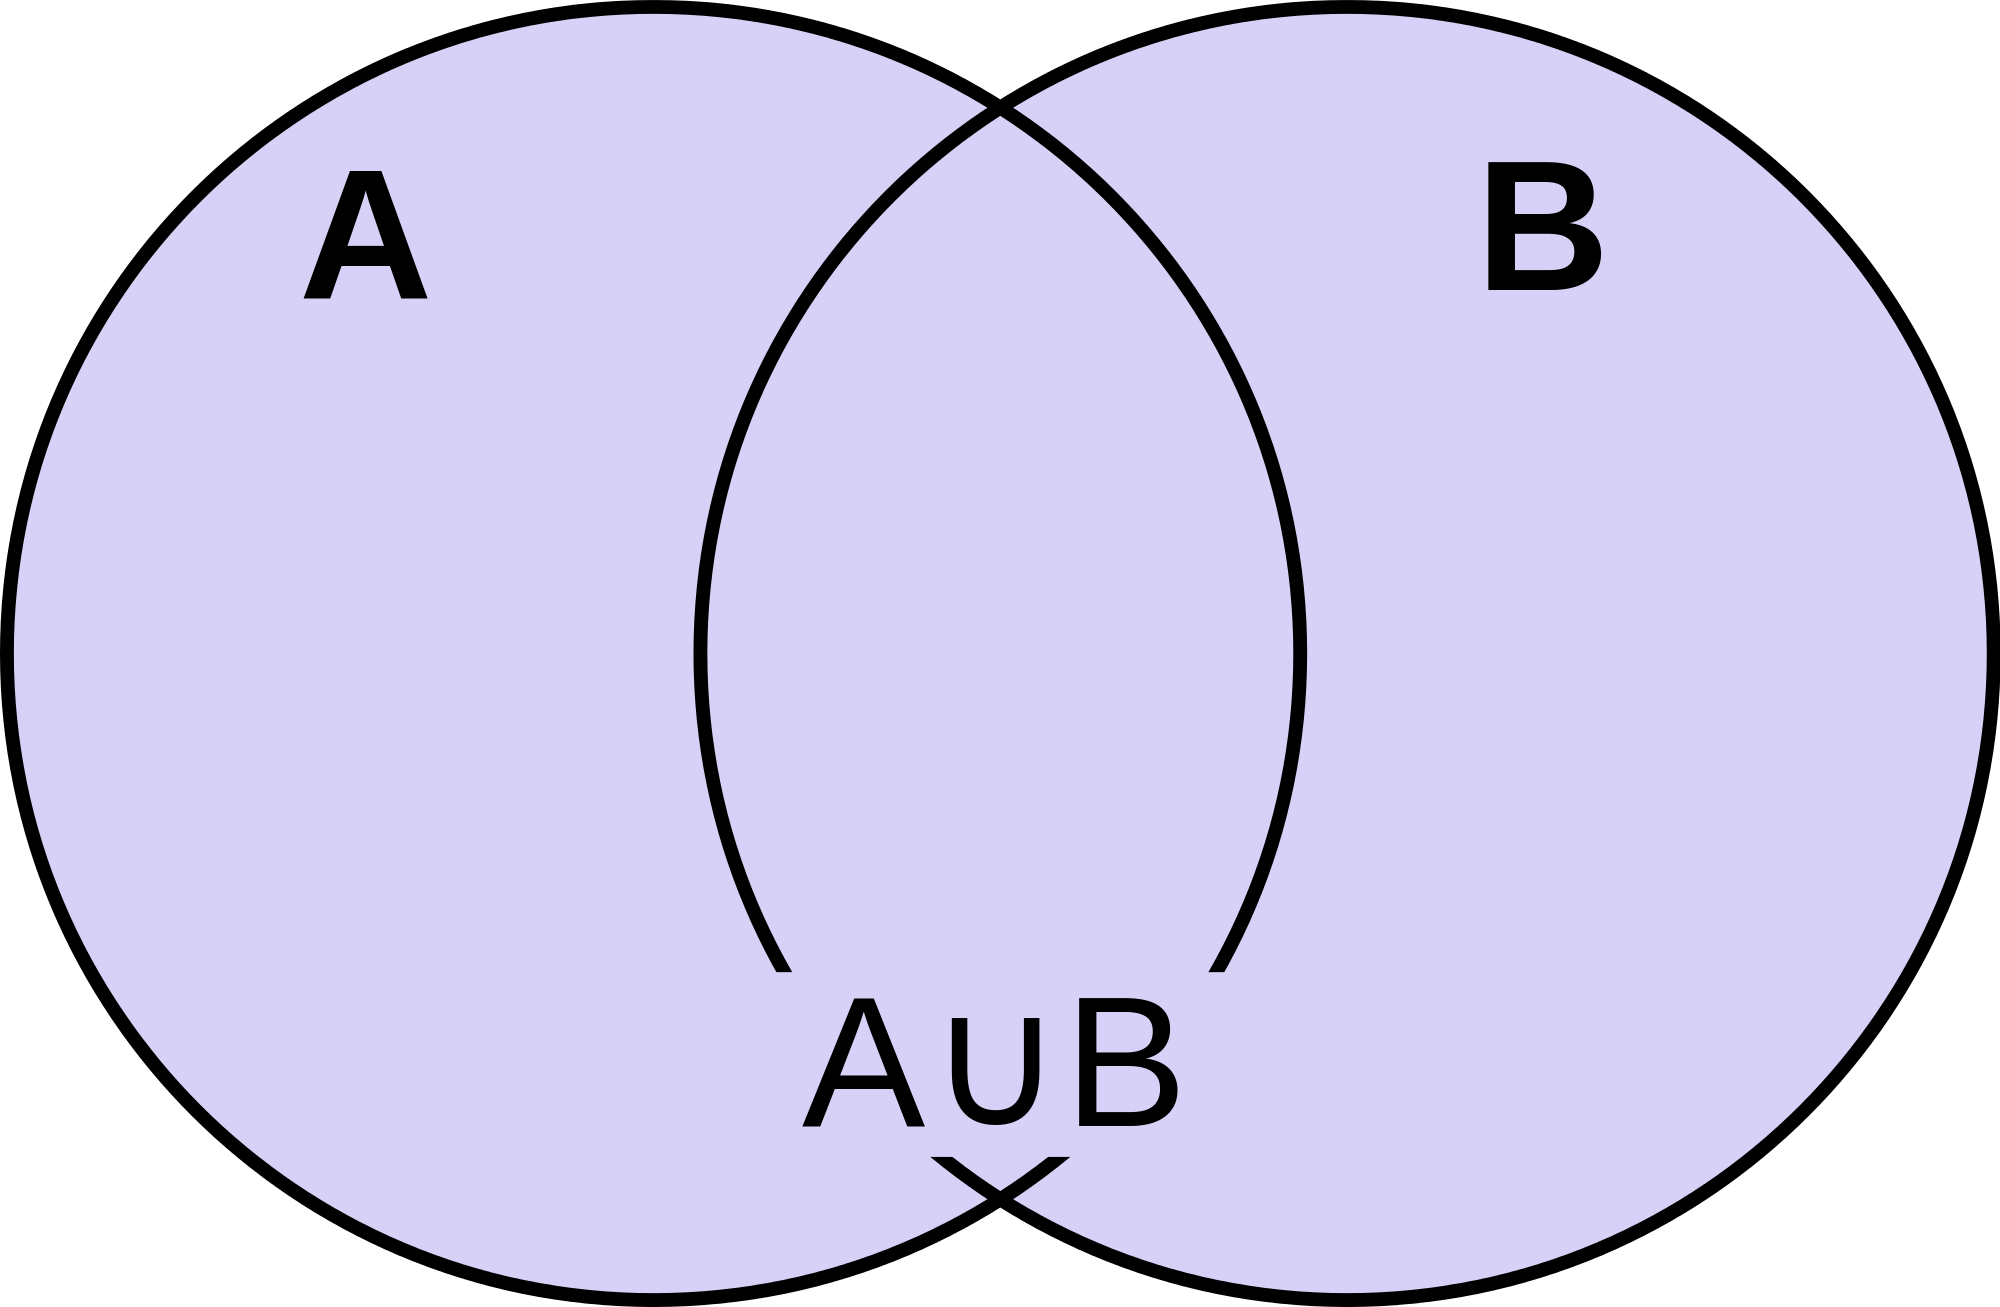
\includegraphics[width=0.3\textwidth]{AunionB}
\caption{Diagrama de Venn de A unión B.} \label{AunionB}
\end{figure}

Si la probabilidad de dos resultados es independiente, es decir que no afecta la una a la otra, entonces la probabilidad de que ambos ocurran está dada por \ref{probabilidadeventosindependientes}.
Esta operación se define como intersección de A y B (se lee <<A intersección B>>) Un ejemplo claro de intersección es el lanzamiento de dos monedas.
La probabilidad en un lanzamiento de que salga cara es de 1/2, por lo tanto la probabilidad de que en las dos monedas salgan cara al mismo tiempo es de 1/4 (claramente los resultados no se afectan entre sí ya que el resultado en uno de los lanzamientos no condiciona para nada al segundo de ellos)

\begin{equation}\label{probabilidadeventosindependientes}
p(A \cap B) = p(A) \cdot p(B)
\end{equation}

\begin{figure}[H]
\centering
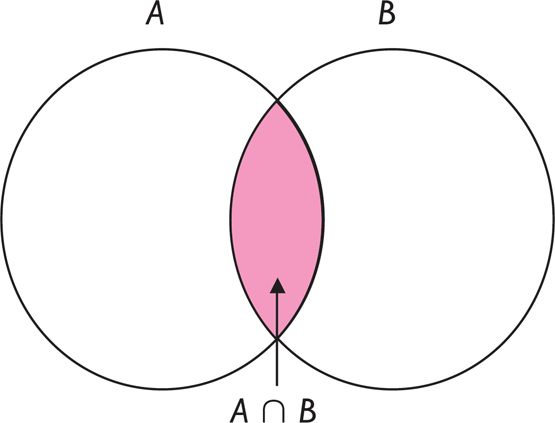
\includegraphics[width=0.3\textwidth]{AinterseccionB}
\caption{Diagrama de Venn de A intersección B.} \label{AinterseccionB}
\end{figure}

Finalmente, si A y B son dos sucesos, la probabilidad de que ocurra B dado A (es decir que A ocurre antes que B) se denota por p(B $\mid$ A) y es llamada probabilidad condicional y viene dada por ~\ref{probabilidadcondicionada}.

\begin{equation}\label{probabilidadcondicionada}
p(A \mid B) = \frac{p(A \cap B)}{p(B)}
\end{equation}

\section{Variables Aleatorias.}

En contraposición a los eventos discretos, en un caso el seguimiento y la captura de movimiento, estamos más interesados en la aleatoriedad asociada a suceso como pueden ser la variación de una señal eléctrica o al movimiento de una persona (son eventos que se dan en un espacio continuo de tiempo).
En este caso podemos pensar en el elemento de interés como una variable aleatoria en un espacio continuo de valores como ya aclaramos anteriormente.
Una variable aleatoria es básicamente una función que mapea todos los puntos en el espacio de muestra a los números reales. 
Por ejemplo, la variable aleatoria continua $X(t)$ que podría mapear tiempo con respecto a posición, en cualquier instante de tiempo $t$ debería decirnos la posición esperada en dicho instante de tiempo.
Las variables aleatorias pueden ser discretas, cuando se puede contar el conjunto de los resultados posibles, o continuas, cuando toma valores en una escala continua lo que significa que el número de resultados posibles es infinito.

Una definición más formal de todo lo enunciado anteriormente, es que una variable aleatoria es una función del espacio muestral $\Omega$ en el conjunto de los números reales.
Las variables aleatorias se denominan generalmente X, Y, Z o con otra letra mayúscula escogida del del final del alfabeto. Por ejemplo, 

\begin{center}
\centering
X:$\Omega$ $\to$ R
\end{center}

define la variable aleatoria X como una función del espacio muestral en el conjunto de los números reales.

Las variables aleatorias se clasifican de acuerdo a su recorrido.
Si el número de valores que puede tomar es finito o infinito numerable (tiene infinitos elementos que pueden ser numerados, como el conjunto de números enteros), X se denomina variable aleatoria discreta. 
Si el recorrido de X es en un conjunto de valores (por ejemplo, los valores de un intervalo de números reales), se denomina variable aleatoria continua.

En el caso de variables aleatorias continuas, la probabilidad de cualquier evento simple discreto A es cero, esto es, P(A)=0.
Una función común que representa la probabilidad de una variable aleatoria, es definida como la función de distribución acumulativa.
Esta función (ecuación \ref{funciondistribucionacumulativa}) representa la probabilidad acumulativa de las variables aleatorias continuas X para todos (los no numerables) eventos hasta x.

\begin{equation}\label{funciondistribucionacumulativa}
F_{x}(x)= p(-\infty,x]
\end{equation}

Algunas importantes características de las funciones de distribución acumulativa son:

\begin{equation}\label{0cuandoxmenosinfinito}
F_{x}(x) \to \textrm{0 cuando x} \to -\infty
\end{equation}

\begin{equation}\label{1cuandoxmasinfinito}
F_{x}(x) \to \textrm{1 cuando x} \to +\infty
\end{equation}

\begin{equation}\label{funcionnodecreciente}
F_{x}(x) \textrm{es una función no decreciente de x} 
\end{equation}

la expresión \ref{funciondistribucionacumulativa} es usada más comúnmente en su forma de su derivada y se conoce como la función de densidad de probabilidad (ecuación \ref{funciondedensidaddeprobabilidad})

\begin{equation}\label{funciondedensidaddeprobabilidad}
f_{x}(x)=  \frac{\textrm{d}}{\textrm{dx}}F_{x}(x)
\end{equation}

La función de la expresión \ref{funciondedensidaddeprobabilidad} presenta las siguientes propiedades:

\begin{equation}\label{funciondensidaddeprobabilidadnonegativa}
f_{x}(x) \textrm{es una función no negativa} 
\end{equation}

\begin{equation}\label{probabilidaddelaintegraldensidaddeprobabilidad}
\int_{-\infty}^{+\infty}f_{x}(x)dx = 1  
\end{equation}

Finalmente la probabilidad en la integral en cualquier intervalo [a,b] está definida como:

\begin{equation}\label{integraldensidaddeprobabilidad}
P(a < X < b) = \int_{a}^{b}f_{x}(x)dx = P(X < b) - P(X < a)
\end{equation}

\section{Media y varianza.}

Al saber la distribución de una variable aleatoria tenemos un conocimiento total sobre ella. 
Sin embargo, en la práctica a menudo es imposible o innecesario conocer la distribución de probabilidad que describe un experimento aleatorio particular. 
En lugar de lo anterior, puede ser suficiente determinar unas pocas cantidades características, como el valor medio y una medida que describa la dispersión alrededor del valor medio (de esta forma se caracteriza en una distribución de probabilidad Normal). 
Muchos de nosotros estamos familiarizados con el concepto de media o promedio de un serie de números. 
La media para un espacio muestral N (se define como espacio muestral todos los posibles resultados de un experimento estadístico,como comentamos en la sección anterior) de una variable aleatoria X, el promedio, la media muestral o esperanza está dada por:

\begin{equation}\label{mediamuestral}
\bar{X} = \frac{X_{1} + X_{2} + \dots + X_{N}}{N}
\end{equation}

La media de una variable aleatoria X, se puede expresar como $\mu_{X}$ o simplemente como $\mu$ cuando sabemos a que variable aleatoria está referido. 
También es común referirse a la media como el valor esperado o esperanza, en cuyo caso se expresa como E(X).

Si X es una variable aleatoria discreta con distribución de probabilidad f(x) la media o valor esperado de X vendría dado de la siguiente forma:

\begin{equation}\label{mediavariablealeatoriadiscreta}
\mu = E(X) = \sum_{x}xf(x) 
\end{equation}

En el caso de que X sea una variable aleatoria continua tendríamos la siguiente expresión:

\begin{equation}\label{mediavariablealeatoriacontinua}
\mu = E(X) = \int_{-\infty}^{+\infty}xf(x) dx
\end{equation}

La varianza es un elemento de gran importancia que caracteriza la distribución de una variable aleatoria. 
Describe la amplitud del recorrido de la variable aleatoria. 
En otras palabras es un término que nos da información sobre la desviación o dispersión que hay con respecto a la media en las muestras usadas para calcular dicha media.
Un ejemplo para explicar el concepto de varianza podría el ruido en una señal senoidal, en este caso la varianza nos daría una idea de la afectación del ruido en dicha señal. 
Para cualquier variable aleatoria X de media $\mu$, la varianza $\sigma^2$ se define como:

\begin{equation}\label{varianza}
\sigma^2 = var(X) = E(X - \mu)^2
\end{equation}

En el caso de que X sea una variable aleatoria discreta, entonces la varianza sería:

\begin{equation}\label{varianzadiscreta}
\sigma^2 = var(X) = \sum_{x}(x-\mu)^2 f(x)
\end{equation}

Por otro lado en el caso de que X sea una variable aleatoria continua, la varianza se definiería de la siguiente manera:

\begin{equation}\label{varianzacontinua}
\sigma^2 = var(X) = \int_{-\infty}^{+\infty}(x-\mu)^2 f(x) dx
\end{equation}

En el caso de que X sea continua la raíz cuadrada de la varianza $\sqrt[]{\sigma^2} = \sigma $, se conoce como la desviación típica o estándar de X.

La varianza en una propiedad estadística muy usada en las señales aleatorias, ya que si se supiera la varianza de una señal que de otro modo fuera supuesta para ser constante alrededor de un valor, la magnitud de la varianza daría una idea de cuanto nos estamos desviando con respecto a la media.
En el filtro de Kalman usaremos la varianza con el fin de saber cuanto ruido hay en nuestra medida o como de deslocalizados nos encontramos en el mapa, este asunto lo trataremos en secciones posteriores cuando hablemos de la propagación del error.

\section{Distribución de probabilidad Normal o Gaussiana}
Esta distribución de probabilidad ha tenido un uso muy extendido en el modelado de sistemas aleatorios por muchas razones.
Introduciremos algunas de ellas para poder caracterizarla. 
Muchos procesos de la naturaleza podrían asemejarse a una distribución normal o estar muy cercana a esta, es decir que se comportan siguiendo una distribución de probabilidad que bien podría ser una normal.
De hecho, bajo unas condiciones concretas, se puede demostrar que una suma de variables aleatorias con cualquier distribución tiende hacia una distribución normal o de Gauss. 
El teorema que define esta propiedad es conocido como el teorema del límite central, y es muy útil para ciertas aplicaciones. 
La distribución Normal o Gaussiana que podemos ver en la figura \ref{distribucionnormal_figura} tiene algunas propiedades que la hacen matemáticamente muy manejable y es uno de los ejes principales sobre los que se postuló el filtro clásico de Kalman.

\begin{figure}[H]
\centering
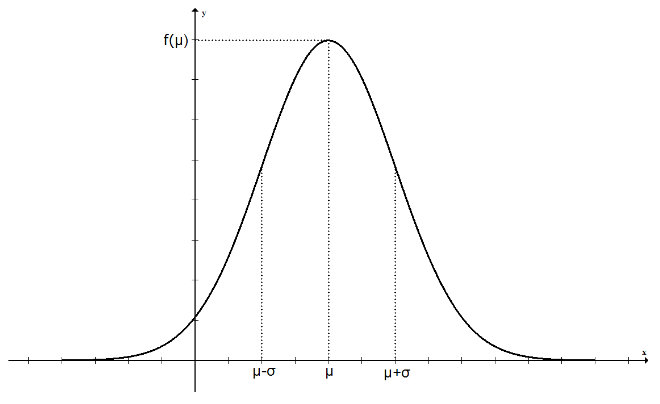
\includegraphics[width=0.7\textwidth]{d_normal_4}
\caption{Función de distribución de probabilidad Normal o Gaussiana.} \label{distribucionnormal_figura}
\end{figure}

La función de densidad de probabilidad de una variable aleatoria X con distribución normal de parámetros $\mu$ y $\sigma$ se define matemáticamente como:

\begin{equation}\label{distribucionnormal}
f(x) = \frac{1}{\sigma\sqrt[]{2\pi}}e^{-(x-\mu)^2/2\sigma^2} , -\infty < x < \infty
\end{equation}

La notación típica para representar los valores de densidad de una variable aleatoria X con media $\mu$ y desviación típica $\sigma$ es $\dist{N}$(X;$\mu$,$\sigma$) aunque en algunos textos también se usa la varianza(no implica ningún problema ya que esta se deriva de la desviación típica). Algunas propiedades de la distribución normal son las siguientes:


1. f(x) es simétrica respecto a x = $\mu$.

2. El máximo de f(x) está en x = $\mu$.

3. Los puntos de inflexión de f(x) están en x = $\mu$ + $\sigma$ y x = $\mu$ - $\sigma$.

Como f(x) es una función de densidad cumple las siguientes propiedades:

\begin{equation}\label{distribucionnormalmayorquecero}
f(x) \geq 0
\end{equation}

\begin{equation}\label{distribucionnormalintegral1}
\int_{-\infty}^{+\infty}f(x)dx = 1
\end{equation}

\begin{equation}\label{distribucionnormalmediaintegral}
\mu = \int_{-\infty}^{+\infty}xf(x)dx
\end{equation}

\begin{equation}\label{distribucionnormalprobabilidad}
P(a \geq X \geq b) = \int_{a}^{b}\frac{1}{\sigma\sqrt[]{2\pi}}e^{-(x-\mu)^2/2\sigma^2}
\end{equation}

La propiedad de la ecuación \ref{distribucionnormalprobabilidad} se da si una cantidad X está normalmente distribuida con parámetros $\mu$ y $\sigma$, en caso contrario no se cumpliría la igualdad ya que no estaríamos tratando con una distribución de probabilidad gaussiana para la cual se define la expresión.

\section{Independencia y Probabilidad condicional}

Podemos ver que en las ecuaciones (\ref{AinterseccionB}) y \ref{probabilidadcondicionada}, que la probabilidad ha sido definida para variables aleatorias continuas. Dos variables aleatorias continuas X e Y son independientes estadísticamente si la probabilidad conjunta $f_{xy}(x,y)$ es igual a la suma de sus probabilidades marginales, es decir, que se consideran independientes si que cumple lo siguiente:

\begin{equation}\label{sucesosindependientes}
f_{xy}(x,y) = f_{x}(x)f_{y}(y)  \longrightarrow P(X \cap Y)
\end{equation}

Un ejemplo algo más claro para ilustrar la independencia sería suponer que lanzamos una moneda dos veces y que dicha moneda no está trucada. Sea A el suceso de que en el primer lanzamiento salga cara y B el suceso de que en el segundo lanzamiento salga cara. Supongamos que A ocurre ¿Cambia eso la probabilidad de que B ocurra?La respuesta lógica que todos daríamos es que no y efectivamente así es. Sabemos que el resultado del lanzamiento de la primera moneda no influye en el resultado del segundo lanzamiento. En el caso de que dos eventos se condicionen entre sí en el cálculo de la probabilidad (sacar bolas de colores de una bolsa) podríamos expresarla de forma matemática. Esta idea se puede expresar matemáticamente usando el concepto de probabilidad condicional que veíamos al principio de esta sección en la ecuación \ref{probabilidadcondicionada} donde expresaríamos la probabilidad de que un evento ocurra cuando previamente ha ocurrido otro.

Otro concepto muy relevante a la hora de hablar de probabilidad condicional es el teorema de Bayes. Para ilustrar la motivación de esta expresión nos remitiremos a un ejemplo expuesto en \cite{Matematicas2004}. Imaginemos que calculamos la probabilidad de que el resultado de un test de VIH realizado sobre un individuo escogido aleatoriamente sea positivo. Para el individuo, es mucho más importante saber si el resultado positivo del test realmente significa que está infectado por el virus. Las probabilidades estaban definidas de la siguiente manera:

\hspace{3.7cm}A = El resultado del test es positivo.

\hspace{3.7cm}$B_1$ = La persona está infectada.

\hspace{3.7cm}$B_2$ = La persona no está infectada.

Estamos interesados en P($B_1$$\mid$ A), es decir, la probabilidad de que una persona esté infectada sabiendo que el resultado es positivo. Las probabilidades P(A$\mid$ $B_1$) y P(A$\mid$ $B_2$) se deducen directamente de las características del test. Ahora queremos calcular las probabilidades condicionales cuando los papeles de A y $B_1$ se invierten.

Antes de calcular la probabilidad en este ejemplo específico, consideraremos el caso más general. Supongamos que los conjuntos $B_1$,$B_2$,$\dots$,$B_n$ forman una partición del espacio muestral $\Omega$, A es un suceso y las probabilidades P(A $\mid$ $B_i$), donde i=1,2,$\dots$,n son conocidas. Lo que queremos calcular son las probabilidades P(A $\mid$ $B_i$). Para la realización del cálculo se procedería de la siguiente manera:

Utilizando la definición de probabilidades condicionales tenemos:

\begin{equation}\label{Pcondicionaejemplo}
P(B_i \mid A) = \frac{P(A \cap B_i)}{P(A)}
\end{equation}

Para calcular $P(A \cap B_i)$, ahora se condiciona sobre $B_i$ :

\begin{equation}\label{Pcondicionaejemplo2}
P(A \cap B_i) = P(A\mid B_{i})P(B_i)
\end{equation}

Por otro lado para evaluar el denominador P(A) se utiliza la ley de la probabilidad total:
\begin{equation}\label{Pcondicionaejemplo3}
P(A) = \sum_{j=1}^{n}P(A\mid B_{j})P(B_j)
\end{equation}

Combinando las expresiones ~\ref{Pcondicionaejemplo},~\ref{Pcondicionaejemplo2} y ~\ref{Pcondicionaejemplo3} se llega a la siguiente expresión, conocida como fórmula de Bayes o teorema de Bayes. Formalmente, siendo $B_{1}$,$B_{2}$,$\dots$,$B_n$ una partición de $\Omega$ y A un suceso. Entonces

\begin{equation}\label{Teoremadebayes}
P(B_{i}\mid A) = \frac{P(A \mid B_{i}P(B_{i}}{\sum_{j=1}^{n}P(A \mid B_{j})P(B_{j})}
\end{equation}

Volviendo al ejemplo, si deseamos calcular P($B_{1} \mid A$), que es la probabilidad de que una persona esté infectada dado un resultado positivo en el test. Una vez el test ha dado positivo la población se divide en dos conjuntos, uno denominado $B_{1}$ en el que la persona está infectada y otro $B_{2}$ en el que la persona no está infectada. Si usamos la expresión \ref{Teoremadebayes} que es el teorema de Bayes, tenemos:

\begin{equation}\label{Pcondicionaejemplo4}
P(B_{1}\mid A) = \frac{P(A \mid B_{1}P(B_{1}}{P(A \mid B_{1})P(B_{1}) + P(A \mid B_{2})P(B_{2})}
\end{equation}

De esta manera calcularíamos la probabilidad de que una persona se encuentre infectada sabiendo que el test ha resultado positivo.

Con todos estos conceptos ya tendríamos los suficientes conocimientos como para comprender la base matemática básica sobre la que se formulan los filtros Bayesianos y por supuesto los filtros de Kalman.
El resto de formulaciones matemáticas relacionadas con los filtros Bayesianos las encontraremos en el capítulo \ref{ch:capitulo2} junto con su explicación teórica.
